\begin{figure*}[ht!]
    \centering
    \vspace{-2.6cm}
    \centerline{
        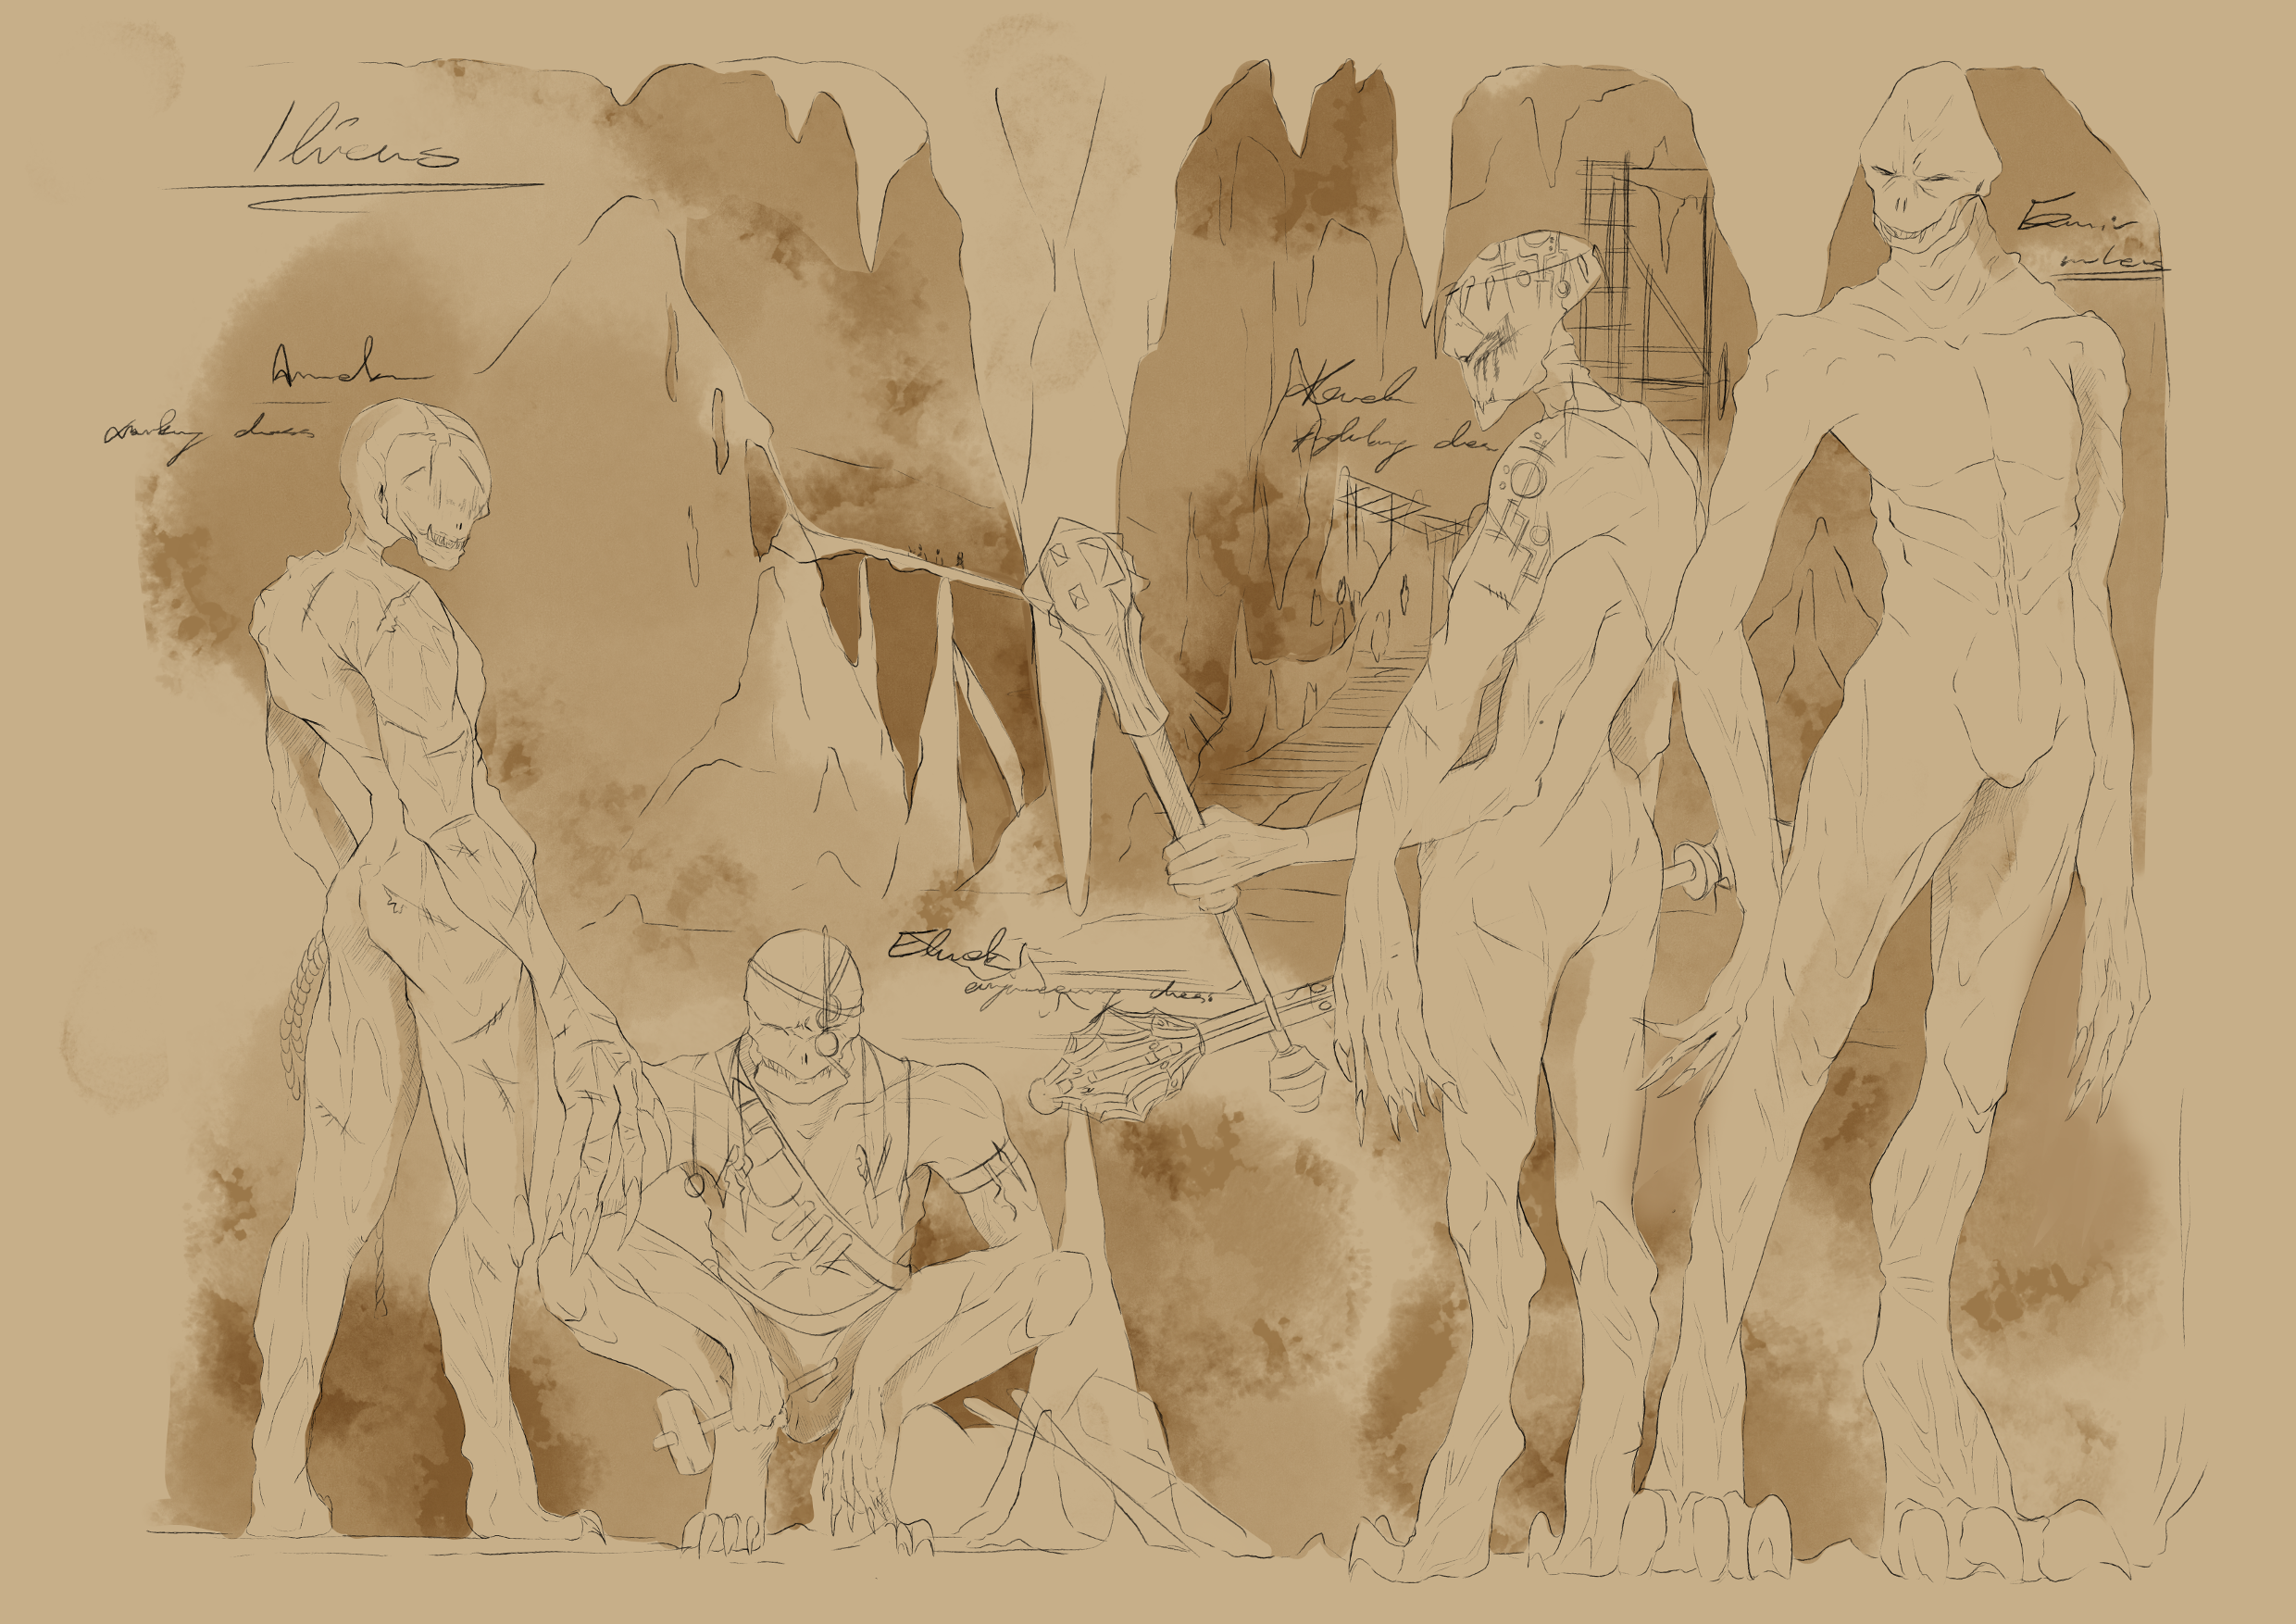
\includegraphics[width=\paperwidth,keepaspectratio]{media/ilians_sm.png}
    }
    \par
    The four castes of Ilian: Arnak (worker), Elnak (engineer), Karek
    (warrior) and Emir (ruler).
\end{figure*}

\subsection{Ilians}
\label{sec:Ilians}

The \emph{Ilians} are a monstrous, humanoid and giant race that live in vast
and great cities deep underground. They are master psionics, and live in a
strictly ordered society.

\subsubsection{Physiology}

The appearance of Ilians varied across the castes, but they all had a few
features in common. Their skin is dark grey or light blue, they are often
above two metres tall, and have no bodily hair. An Ilian has no nose or ears,
but instead simply have small holes were the nose and ears would be on a
regular humanoid. The strength of their senses varies rapidly between the
specific castes. Elnak, for example, have excellent and sharp eyesight, while
the workers drones, the Arnaks, are all blind. And although Arnaks have
excellent hearing and olfactory organs to detect threats, these senses have
atrophied within the ruling cast, the Emir, who instead use their psionic
abilities to perceive their surroundings.

Ilians have only one biological gender, and give birth to live young by
producing a small aquatic, limbless snake out of their mouths. This worm
represents the original and unaltered form from which all Ilians
originated. These young are then fed variations of their only food - Ramesk -
which force them to grow into the various castes of Ilian society. This allows
Ilian societies to engineer exact populations and demographics for each caste
depending on societal needs. Spawns that are fed regular food (such as meat,
vegetables or mushrooms) would turn into Arnaks. Arnaks however were also
capable of producing their own spawns, that could only mature into other
Arnaks. In many Ilian societies the dead were symbolically fed to a new
generation of spawns, allowing them to contribute one last time to their
society. Larger Ilian societies and cities have growth chambers, large glass
tanks filled with Ramesk that facilitated the birth and nurturing of their
young.

\subsubsection{History}

Their early history and origins are shrouded in mystery. Ilians already dwelt
in their great underground cities when the dwarves, elves and humans went
underground during the \nameref{sec:Schism}. The Ilians did not take kindly to
what they perceived as intruders upon their land, and attempted to drive the
humanoid races back to the surface.

Although the Ilians had a massive advantage, as their cities and war
infrastructure was already built, their slow reproductive cycles and strict
and unmoving societal structure ultimately caused them massive problems in
the war against the humanoid races.

The dark elves, dwarves and deepkin fought the Ilians relentlessly in an
attempt to establish themselves in the deep. And although early conflicts and
wars often ended in favour for the Ilians, the tide turned against them when
the deepkin began building \hyperref[sec:Everblack Golem]{everblack golems}
that could withstand the psionic powers of the Ilians. These constant battles
and conflicts cost both sides heavily, and ultimately culminated in the
downfall of the Ilian culture and society across most of Aror. The victory was
devastating for the humanoids as well, and it lead to a \hyperref[sec:Exodus
  from the Depths]{great exodus from the depths} for many deep dwelling
humanoids.

Nowadays only ruins remain where once proud Ilian cities stood. Burying their
psionic machinery, artefacts and riches beneath them. Some communities and
cities have survived and guard their treasures still, while some retreated
deeper underground into solitude and isolation.

\subsubsection{Society}

The Ilian society was strictly ordered into castes, where the members of each
caste had distinct biological traits suited for the work they were required to
perform. There were four main casts: \emph{Arnak}, \emph{Elnak}, \emph{Karek},
and \emph{Emir}.

Ilian also have their own language, called \emph{Ilian} which had no writing
system. Ilians transmitted their thoughts, feelings or knowledge as psionic
energy through telepathy or inscribed them into
\hyperref[sec:Everblack]{everblack} crystals, which could then be accessed by
any psionic individual. The language ``Ilian'' was invented by the Elnak, to
allow individual Ilians to talk to other races through telepathy. Many Ilians
did not talk with each other, and simply use their psionic powers to command
or force those of a lower caste to do their bidding.

Ilians are one of the great societal architects, city builders and engineers
of Aror. Ilian cities are built out of carefully hewn stone, and kept together
by a special cement-like mortar that gives their buildings the structural
integrity to support large towering buildings. Their structures thus encompass
multiple levels, and built within large, and wide natural caverns. The centre
almost always features a tall spire, which houses the Emir, Karek and the
higher ranks of the Elnak. On the outlying areas are workshops, farms, storage
facilities and smaller community housing to support the needs of the
city. Often larger settlements will have outlying farms, mines or military
outposts detached from the city depending on the position of natural resources
or strategic locations. These are often overseen by Elnaks in case of farms
and mines, while Karek oversee military outposts. Yet both are always
bolstered by Arnaks that provide support, labour, and defence.

Ilian cities are always covered in a hue of soft green light, as the Elnak
engineers use dim glowing psionically charged Everblack as ambient
lighting. Even though they can all see in the dark (and Arnak cannot see at
all), the soft light helps them distinguish colours. Often their machinery,
artefacts and contraptions powered by psionic magic work to this day, even
though many of their cities have fallen to ruin.

\subsubsection{Ramesk}
\label{sec:Ramesk}

Ramesk is a blueish, thick fluid that the Ilians drank as nourishment. It has
almost no smell, but tastes salty, due to the high mineral content of the
liquid. It was made out of various roots, herbs and mushrooms that grew in the
depths, and was the mainstay food for all Ilian caste members. Although the
Ilians still had humanoid mouths and could eat and digest other food, Ramesk
turned into the main source of nourishment when food became scarce during the
aeon of strife. Not all Ramesk is made equal, and several varying recipes
exist. For example there is a ``Royal Ramesk'', a specialised recipe that
allows Ilian spawns to grow into Emir.

\subsubsection{Arnak}
\label{sec:Arnak}

Arnaks are labourers and front-line warriors, and thus lowest caste of Ilian
society. They stand roughly two and a half metres tall, their bodies are
extremely muscular, and they have sharp claws and teeth they used for hunting
and defending the Ilian cities and outlying farms. They are blind, and rely on
their fine sense of smell and their ability to sense small tremors to move
about in the dark caves.

They are the least intelligent of all Ilians, and were only used as front line
troops, for carving new tunnels, constructing new buildings or tending to
underground farms. Groups of Arnaks were often overseen and psionically
controlled by Karek or Elnak, who could force them into hibernation if their
labour was not needed, or food had to be rationed or preserved. Arnaks were
also to reproduce on their own by gestating a special lesser spawn, which was
vital to replenish their numbers in the field or in remote workshops and
farms.

As the most numerous of all the Ilians, they can still be found underground
today, often leaderless and organised into small groups. Their fierce strength
and uncanny senses make them expert hunters of anything that ventures or lives
down below. The fall of major Ilian civilisations and cities have left them
cut off from their supply of Ramesk, and have thus resorted to drinking
humanoid blood, which is similar in composition to Ramesk. If no suitable
sources of nourishment are available, Arnaks hibernate beneath
stalactites. The mineral rich water that drops from the stones nourishes them
while they hibernate. Since these wild Arnaks no longer have any access to
Ramesk, or farms to grow food for their young, they forced them to feed their
spawns mushrooms growing in the deep. If no mushrooms or other suitable flora
is available, they hunt living creatures, such as deep dwelling humanoids, to
provide nutrition for their spawn.

Arnaks are now a major scourge of anyone who ventures underground, and many
cultures use Arnaks as the ``boogey man'' to frighten and scare children away
from caves.

\subsubsection{Elnak}
\label{sec:Elnak}

Elnak are the tinkerer and crafter caste of the Ilians. Highly intelligent,
although shorter than any other Ilian. They stood roughly two metres tall, and
had extra-ordinarily sharp eyesight and dexterity to allow them to work on
intricate psionic machinery. They were leaner than other Ilians, but made up
for their lack of strength with advanced psionic powers and abilities. They
were responsible for forging all psionic artefacts and machinery used by the
Ilians.

As the engineers of the Ilian society, they are responsible for a wide variety
of scientific fields and tasks. Elnak's build, research and maintain farms,
engineering workshops, smithies, forges, food processing stations, military
defences as well as the many amenities that are required to keep Ilian society
running.

\subsubsection{Karek}
\label{sec:Karek}

Karek are the elite warrior and fighter caste of the Ilians. They stood between
two and a half, to three metres tall, and had four arms. Highly intelligent
tacticians, powerful psionics, and above all else fierce fighters. There were
but a few Karek per city or community, as they used Arnaks as the main fighting
force. Karek were often high ranking military leaders, akin to captains or
generals, or specialised forces and shook troops.

Some Karek also lead small communities, often by proxy for an Emir. Their
intellect, tactical thinking, and their ability to organise strict hierarchies
allowed to be excellent leaders over smaller communities.

\subsubsection{Emir}
\label{sec:Emir}

Above all others stood the Emir, the ruling caste of the Ilians. Highly
intelligent, and incredibly powerful psionics. They lead their cities
administratively as well as spiritually. Emir were also active in psionic
research, and were brilliant engineers and responsible for leading and
building entire Ilian communities and societies. They towered over three
metres tall, so that they could easily be identified as the rulers by all
other Ilians.

Emir used their psionic powers to levitate and wield a ceremonial
quarterstaff that is a representation of their power within society. Emir are
incredibly powerful psykers, capable of reshaping reality if it so suits
them. Emir are the only ones capable of giving birth to an higher Ilian
spawn. Higher spawns, as compared to the Arnak spawns, were the stock out of
which other Elnak, Karek or Emir were bred.
